\begin{figure}[t]
\centering
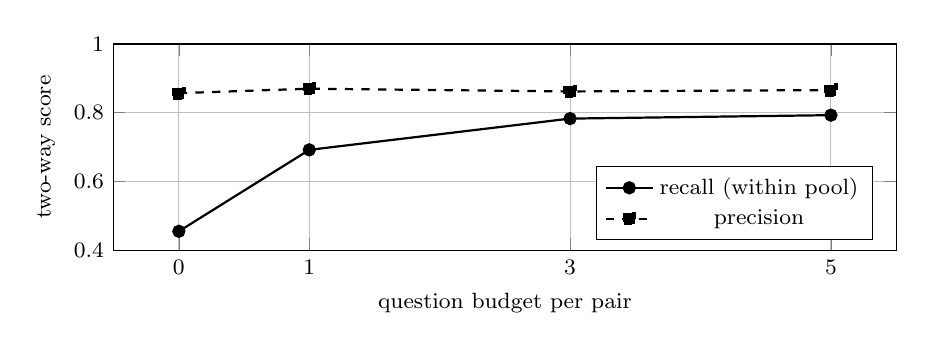
\begin{tikzpicture}
\begin{axis}[width=0.95\columnwidth, height=4.2cm, xlabel={question budget per pair}, ylabel={two-way score}, xtick={0,1,3,5}, ymin=0.4, ymax=1.0,
legend style={at={(0.97,0.05)}, anchor=south east, font=\footnotesize}, tick label style={font=\footnotesize}, label style={font=\footnotesize}, grid=major]
\addplot[mark=*, thick] coordinates {(0,0.455) (1,0.692) (3,0.783) (5,0.793)};
\addlegendentry{recall (within pool)}
\addplot[mark=square*, thick, dashed] coordinates {(0,0.857) (1,0.870) (3,0.862) (5,0.866)};
\addlegendentry{precision}
\end{axis}
\end{tikzpicture}
\caption{Two-way introductions as the question budget grows (gpt-oss-20b, 3,289 pairs). The first question gives most of the gain; precision does not drop.}
\label{fig:budget}
\end{figure}